

\documentclass[twocolumn,10pt,a4j]{ltjsarticle}
\usepackage{kougai}
\usepackage{bxjacalcux}

\title{民俗芸能育成問題における小学生向け学習教材の開発}
\author{1932102 永塚 迅一  指導教員 須田 宇宙 准教授}
\date{}
\begin{document}
\maketitle
\section{はじめに}

%背景
日本には今もなお,人々を魅了し感動を与える伝統芸能がある.伝統芸能には,歌舞伎,能楽,文楽,古典落語などがあり,
その多くは明治時代以前に大成したものである.
しかし,高齢化や後継者不足の問題がある.

伝統芸能の中に,地域の特色が強く入り,地域ごとに伝承されている民俗芸能がある.
地元の民俗芸能に「女沼のささら」という「太夫獅子」「女獅子」「後獅子」の3頭からなる獅子舞があり,毎年11月中旬に女沼香取神社の秋季大祭で披露される\cite{suda2018}.女沼のささらは,ささら保存会によって保存継承がされている.


%問題点
地元小学校の運動会では,4年生から6年生の選抜された代表児童を中心に全員参加でささらを踊る.
そこでささら保存会が運動会前に,代表児童に数回指導を行うのだが,保存会の人数は年々減ってきており,代表児童に対して十分な指導ができないという問題点がある.
同様に,全国の主要な伝統芸能も同じ問題をかかえていると考える.

%目的
そこで本研究では,ささらの踊りを学習できる教材を開発し,保存会の教えと併用することでささら代表児童に十分な踊りの知識を提供することを目的とする.
そして本教材の有用性を示し,全国の伝統芸能にも同様の教材を用いて学習することが,育成問題解決に繋がることを示したい.

\section{ささら学習教材}
本教材は,個人でささらの踊りの学習を進めることができるWeb教材である.工夫した点は,主に良い例と悪い例の動画や写真を用いて解説し,児童に踊りのポイントを意識させて,理解しやすくした点である.

大まかに,太鼓のたたき方などの「基本」,実際に運動会で踊る「出羽」「平庭」の3つを選択できる構成とした.
この内,基本では,良い例と悪い例の動画と写真を用いて解説し,ささらを踊る上で必要な6つの動作を学習してもらう.



\begin{figure}[htbp]
 \begin{minipage}{0.5\hsize}
  \centering
  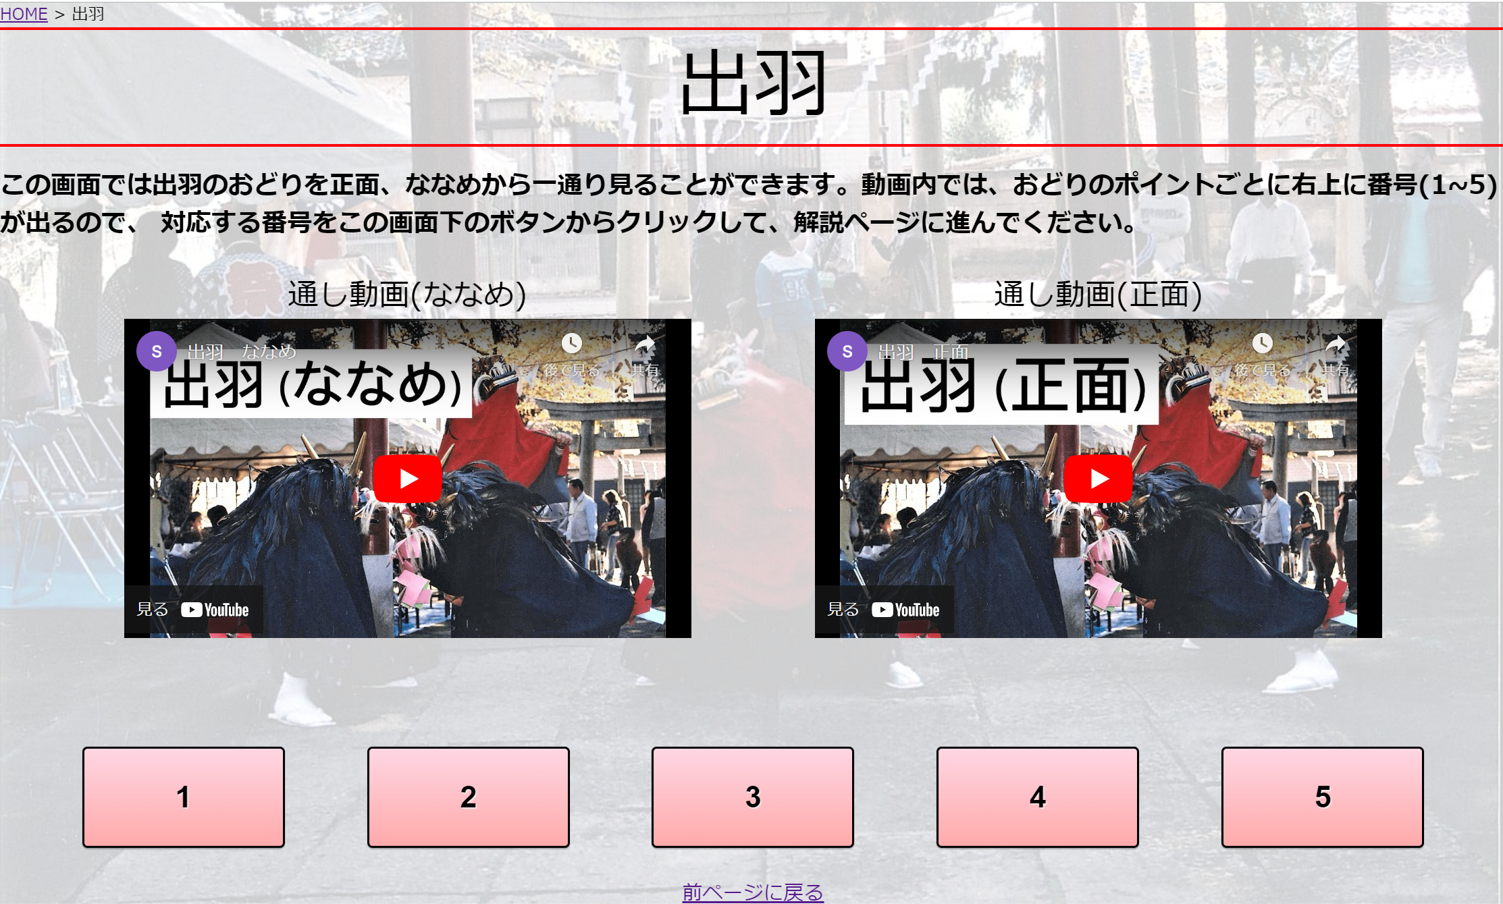
\includegraphics[width=42mm]{figures/zu11.png}
  \caption{出羽の通し動画画面}
   \label{fig:図1}
 \end{minipage}
 \begin{minipage}{0.5\hsize}
  \centering
  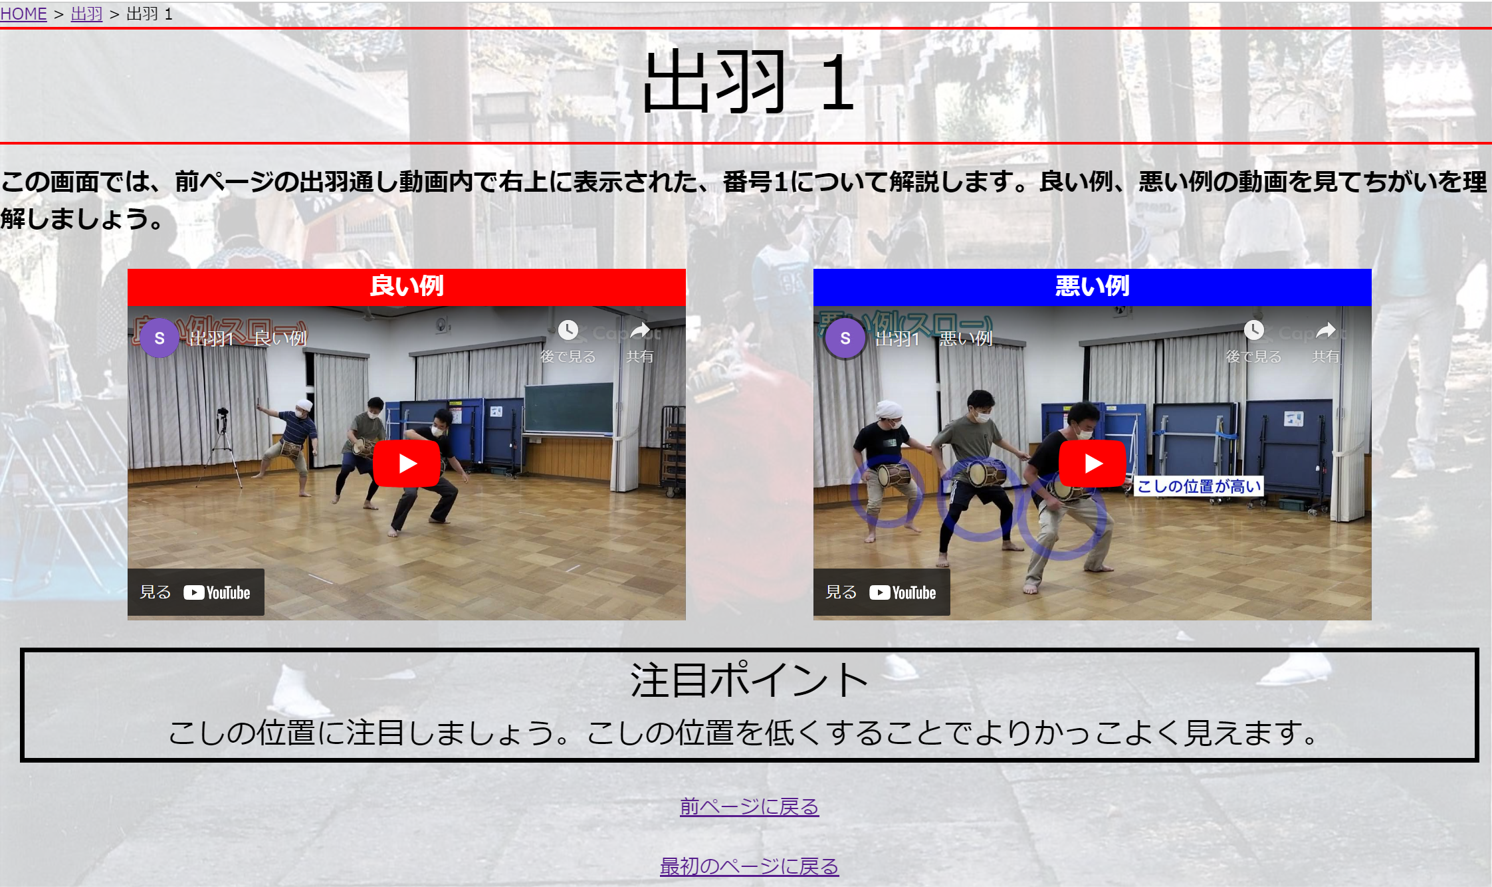
\includegraphics[width=42mm]{figures/zu12.png}
  \caption{出羽の解説ページ画面}
   \label{fig:図2}
 \end{minipage}
\end{figure}

出羽の画面を図\ref{fig:図1}に示す.
上段に説明文を,中段左に斜めからの映像を,中段右に正面からの映像を,下段に解説ページへのリンクを設置している.
はじめに2視点の踊りの通し動画を学習者に視聴してもらう.
出羽の場合,5つのポイントを設定しており,動画内右上にポイント番号が出現する.
出現した番号と対応する番号を,下段に提示してあるリンクから選択することで図\ref{fig:図2}に示す解説ページに遷移する.
解説ページでは,上段に説明文を,中段左に良い例の映像を,中段右に悪い例の映像を,下段に学習者に注目してほしい点を提示している.
平庭も出羽と同じ構成として,4つのポイントについて解説している.



\section{アンケート調査}
本教材の有用性を示すために,小学6年生のささら代表児童5名にアンケート調査を実施した.アンケートは全9項目あり,大きく分けると,
教材の使いやすさ,工夫した点の評価,実用的の3種類について調査した.
図\ref{fig:図3},\ref{fig:図4}は,本研究の有用性を最も示した結果である.
\vskip\baselineskip
\begin{figure}[h]
\begin{center}
 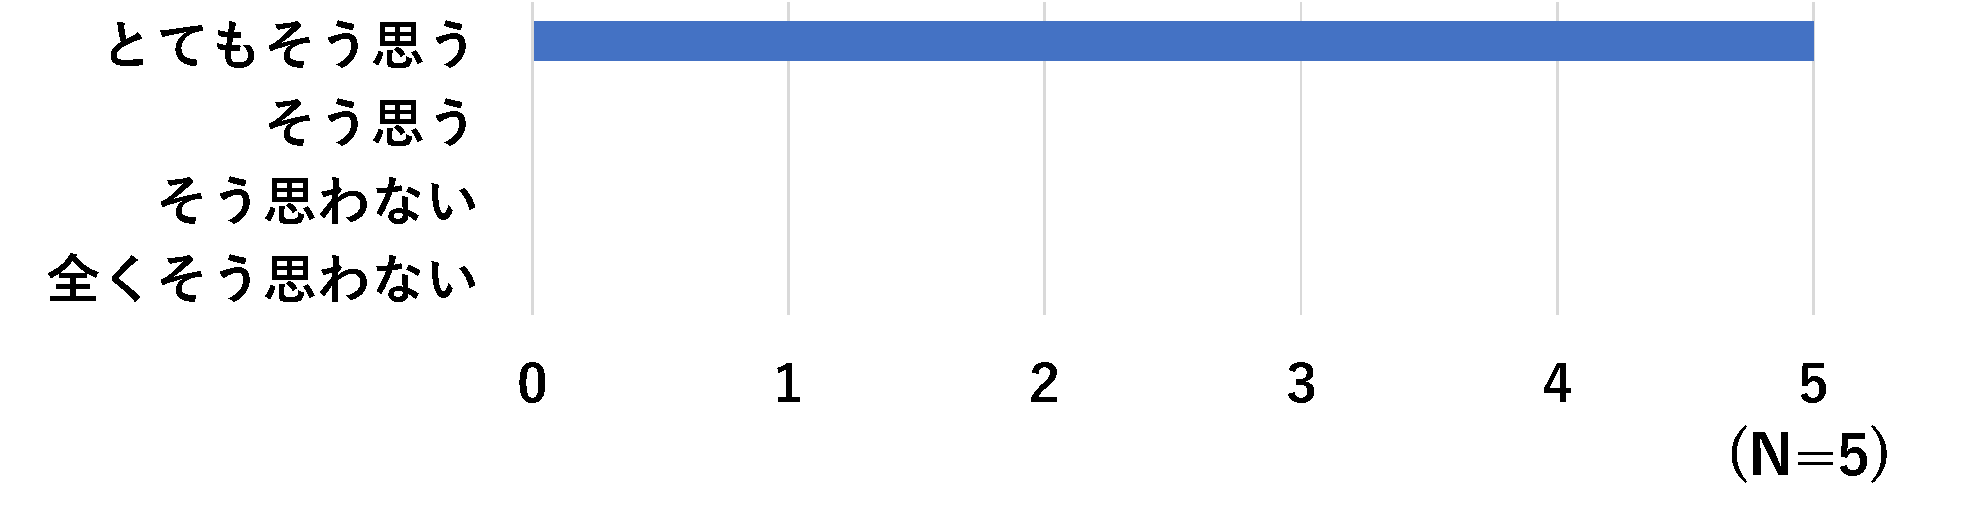
\includegraphics[clip,width=80mm]{figures/zuu3.pdf}
\end{center}
 \caption{良い例と悪い例を用いて解説しているページで\\十分なおどりの情報を得ることができましたか}
 \label{fig:図3}
\end{figure}
\vskip\baselineskip
\begin{figure}[h]
\begin{center}
 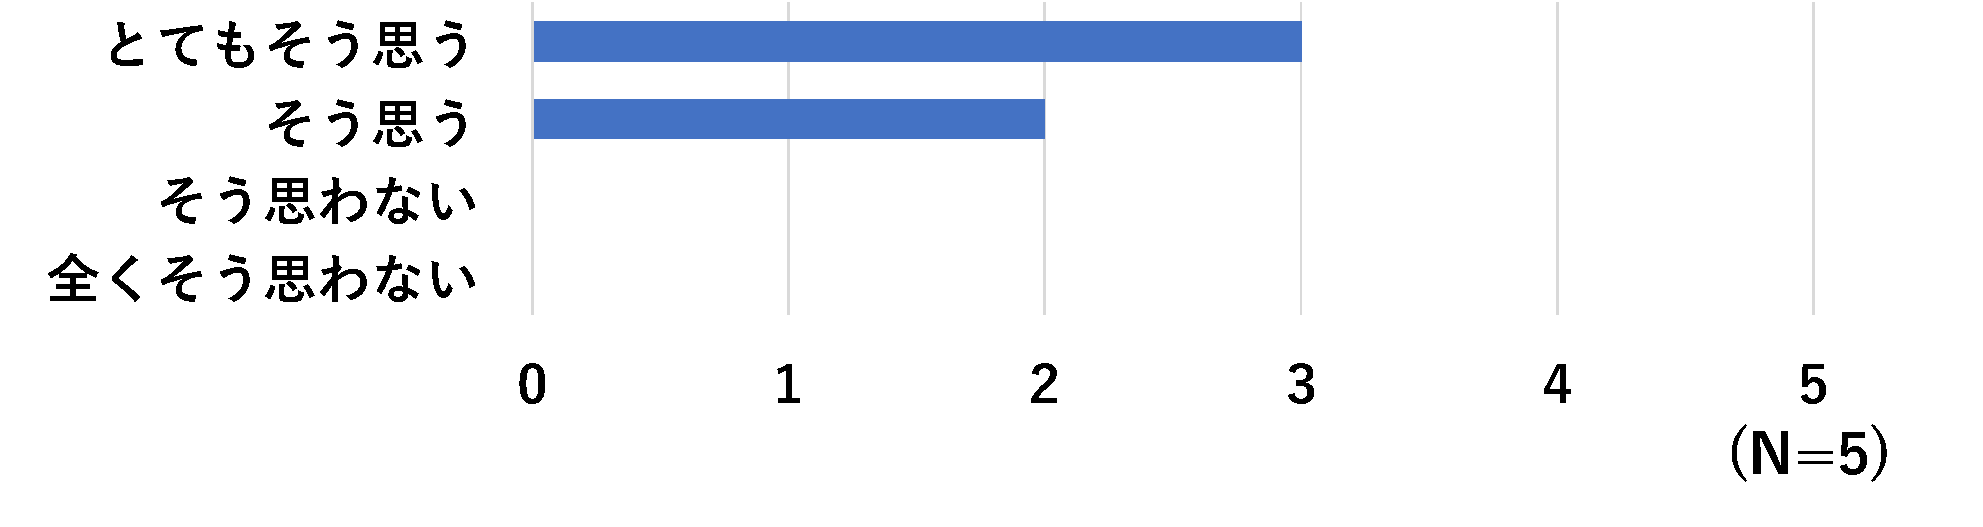
\includegraphics[clip,width=80mm]{figures/zuu4.pdf}
\end{center}
 \caption{ささら保存会の教えと,ささら学習教材を\\組み合わせれば今までより上手におどれると思いますか}
 \label{fig:図4}
\end{figure}

図\ref{fig:図3}より,良い例と悪い例を用いて解説すると十分な踊りの知識を得ることが可能なことが分かる.そして図\ref{fig:図4}から,低評価がなく
代表児童に対して本教材の有用性を示したといえる.よって本研究の目的が達成されたことが分かる.

\section{終わりに}
本研究では,地元の民俗芸能が抱える問題を解決する学習教材を作成し,アンケート調査を実施して有用性を示した.
全国の主要な伝統芸能に対しても,良い例,悪い例を用いたビデオ学習教材を作成することによって解決の糸口になると考える.

\begin{thebibliography}{99}
\bibitem{suda2018} 古河市 生涯学習課: ``女沼のささら(市指定文化財)/古河市公式ホームページ'', \url{https://bunkashisan.ne.jp/bunkashisan/08_ibaraki/7040.html}, 2022/8/8 参照
\end{thebibliography}

\end{document}
